Os guindastes s�o fundamentais em canteiros de obras, no manejo de materiais pesados como vigas de a�o. A figura ilustra uma sequ�ncia de est�gios em que um guindaste i�a uma viga de a�o que se encontra inicialmente no solo. 

\begin{figure}[h]
\centering
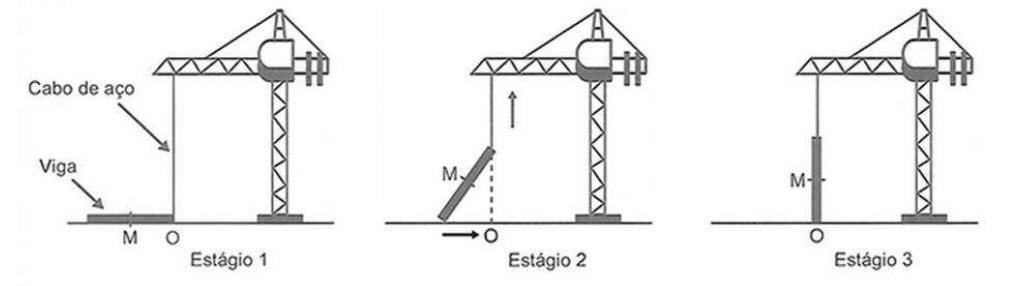
\includegraphics[width=8cm]{../figuras/q155(1)-2018.png}
\end{figure}

Na figura. o ponto O representa a proje��o ortogonal do cabo de a�o sobre o plano do ch�o e este se mant�m na vertical durante todo o movimento de i�amento da viga, que se inicia no tempo t = O (est�gio 1) e finaliza no tempo t, (est�gio 3). Uma das extremidades da viga � i�ada verticalmente a partir do ponto O, enquanto que a outra extremidade desliza sobre o solo em dire��o ao ponto O. Considere que o cabo de a�o utilizado pelo guindaste para i�ar a viga fique sempre na posi��o vertical. Na figura, o ponto M representa o ponto m�dio do segmento que representa a viga. 
O gr�fico que descreve a dist�ncia do ponto M ao ponto O, em fun��o do tempo, entre t = 0 e $t_t$, � 

\begin{figure}[h]
\centering
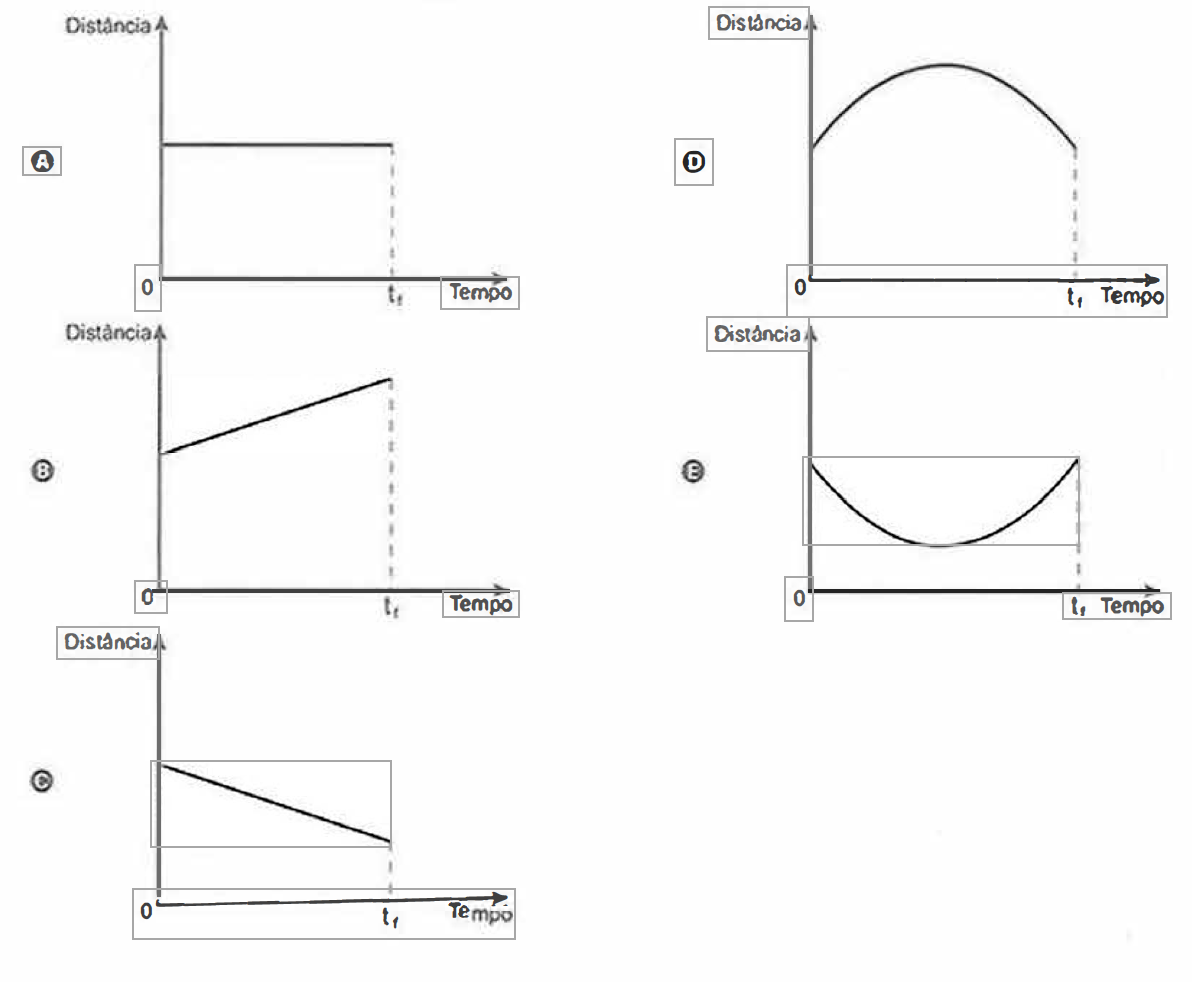
\includegraphics[width=9cm]{../figuras/q155(2)-2018.png}
\end{figure}

\begin{enumerate}
\item[a)]a
\item[b)]b
\item[c)]c
\item[d)]d
\item[e)]e
\end{enumerate}